\title{Fast dictionary learning for high-dimensional seismic reconstruction}
\renewcommand{\thefootnote}{\fnsymbol{footnote}}
%\author{Hang Wang, Quan Zhang, Wei Chen, Xingye Liu, Shaohuan Zu, and Yangkang Chen
\author{Hang Wang, Wei Chen, Quan Zhang, Xingye Liu, Shaohuan Zu, and Yangkang Chen
\thanks{H. Wang, Q. Zhang, and Y. Chen are with the Key Laboratory of Geoscience Big Data and Deep Resource of Zhejiang Province, School of Earth Sciences, Zhejiang University (chenyk2016@gmail.com).}
\thanks{W. Chen is with the Key Laboratory of Exploration Technology for Oil and Gas Resources, Ministry of Education, Yangtze University, and also with the Hubei Cooperative Innovation Center of Unconventional Oil and Gas, Yangtze University.}
\thanks{X. Liu is with College of Geology and Environment, Shaanxi Provincial Key Laboratory of Geological Support for Coal Green Exploitation, Xi'an University of Science and Technology.}
\thanks{S. Zu is with College of Geophysics, Chengdu University of Technology.}
\thanks{The research is supported by the starting fund from Zhejiang University and the National Natural Science Foundation of China (Grant No. 41804140), the Open Fund of Key Laboratory of Exploration Technologies for Oil and Gas Resources (Yangtze University), Ministry of Education (Grant No. PI2018-02). (Corresponding author: Yangkang Chen.)}}
\maketitle

%, college of geology and enviroment
%58 Yanta road
%Beilin district

\begin{abstract}
A sparse dictionary is more adaptive than a sparse fixed-basis transform since it can learn the features directly from the input data in a data-driven way.  However, learning a sparse dictionary is time consuming because a large number of iterations are required in order to obtain the dictionary atoms that best represent the features of input data. The computational cost becomes unaffordable when it comes to high-dimensional problems, e.g., 3D or even 5D applications. We propose an efficient high-dimensional dictionary learning method by avoiding the singular value decomposition (SVD) calculation in each dictionary update step that is required by the classic K-singular value decomposition (KSVD) algorithm. Besides, due to the special structure of the sparse coefficient matrix, it requires a much less expensive sparse coding process. The overall computational advantage of the new dictionary learning method is very decent while the results are still comparable or event better than those from the traditional KSVD method. We apply the proposed method to both 3D and 5D seismic data reconstructions and demonstrate the successful and efficient performance.
\end{abstract}

\begin{keywords}
Seismic data reconstruction, signal processing, dictionary learning, high-dimensional problem
\end{keywords}

\section{Introduction}
The seismic acquisition in the field will inevitably come across many problems that affect the completeness of collected data \cite{Chao2018Adap}. The huge expense of acquisition is one of the most important reasons for this degradation. In order to minimize the cost, the acquisition system is always not dense enough, which will generate a too sparse data set. Additionally, the topography in working area is usually complex, and the deployment of receivers will be limited in certain places. As a result, the reflection information from these areas cannot be sufficiently obtained. In addition to the problems mentioned above, there are many anomalous traces caused by the defective instruments and erratic noise in the raw data. Simply removing them will also lead to the considerable loss of seismic traces. This information loss may cause some troubles in the following processes, such as inversion and migration. Reconstructing these missing traces is very meaningful to the accurate imaging of subsurface structures. The original data from field acquisition are usually five-dimension volumes \cite{yangkang2016irr5d,jianjun2017five}, including inline, xline, azimuth, offset and time dimensions. The reconstruction of the missing traces can provide much more information than the conventional 2D or 3D data interpolation. 

\old{The random noise is another important reason for decreasing data quality, and will also cause problems in the subsequent processes ?. Thus, the random noise should also be eliminated properly to generate a good imaging result. Fortunately, the interpolation and denoising of seismic data have some similar features and can be dealt with by the similar mathematical methods, such as prediction-based method ?, transform-based method ? and rank-reduction-based method ?, and so on.}Prediction-based method is often used as an effective tool for the denoising and interpolation of seismic data. It designs a prediction filter in the frequency-space domain. Then, in each frequency slice, the filter is applied to suppress random noise or interpolate the missing traces \cite{Spitz1991fx,Guochang2019Multi}. \old{? first proposed the idea that the linear events are predictable. He used the Wiener method to derive a filter and applied it to attenuate the random noise in each frequency-space slice. ? continued applying this idea to interpolate the under-sampled seismic data. This method shows good robustness even if the seismic data contains non-linear events and unstable amplitude. ? utilized a narrow-band model to interpolate the sparse data collected in the field, aiming at saving the cost of acquisition. Different examples all demonstrated the validity of this method. ? treated the seismic data as two parts, i.e., non-aliased part and aliased part. The low-frequency components corresponding to the non-aliased part are reconstructed first by the minimum-weighted norm method. Then, this part was used to extract the prediction filter. The method in this step is called multistep autoregression. The extracted filter is then applied to the whole data to interpolate the missing traces in all frequency components. This algorithm shows outstanding performance in reconstructing irregular data. ? designed a non-stationary method to interpolate the near offset data. Compared to the traditional method that simply uses pseudo-primaries to replace the missing data, this method can effectively reduce the negative artifacts caused by the multiples. Both 3D synthetic data and 2D examples showed its superiority over the conventional method.}Transform-based methods are commonly used approaches for seismic interpolation and denoising \cite{Trad2002rt,Abma2006pocs,Side2010damped}. \old{? proposed a two-step method based on the Fourier transform. Firstly, it reconstructs the data in the low and non-aliased frequencies. This reconstructed part is then used as a prior information to recover the high and aliased frequency components. This process is implemented in an inversion framework with a penalty. To meet the linear assumption, this algorithm needs to be implemented in local windows. ? added the sparseness constraint to the frequency slices of the five-dimensional data. This high-dimensional reconstruction algorithm can preserve the variation information of reflected amplitude and minimize the artifacts caused by the method itself.  ? regarded the interpolation of seismic data as an inversion problem. They used dreamlet transform to interpolate the missing traces, based on the projection onto convex sets (POCS) framework. The data examples showed that the dreamlet-based method has better ability to recover the missing signals than the curvelet-based one. ? used seislet transform as the sparse constraint, and analyzed the difference between the POCS and iterative shrinkage thresholding (IST) methods in different cases. Some real marine data and synthetic examples demonstrated its good performance in the sparse representation of the under-sampled data.} Rank-reduction-based methods are mainly based on the assumption that the complete and incomplete data correspond to the low-rank and high-rank features, respectively. A good separation of the rank values can provide proper reconstructed results of under-sampled seismic data \cite{Jianjun2013rank,Yangkang2016drr,yangkang2019nc}. \old{? formed the high-order tensor using the noisy and under-sampled high-dimensional data, and obtained the singular value decomposition of this tensor to reduce the rank of it. This method can effectively recover the synthetic and field data with random noise and missing traces even if the event shapes of them are complex. ? reconstructed the noisy and incomplete five-dimensional data by the damping operator which can better distinguish the noise and recover the missing traces more accurately. ? continued to propose an optimally damped operator which simultaneously keeps the advantages of both optimal weighted and damping operators. The simultaneous interpolation and denoising result of it is more accurate than the conventional method that just has one operator.}

In addition to the popular methods mentioned above, dictionary-learning-based (DL) methods are recently developed rapidly for the denoising and reconstruction of seismic data \cite{lingchen2015multiscale,Siahsar2017multitask,yangkang2020sgk}. This novel method can commonly be divided into two steps: the sparse coding and the dictionary update. The two parts are implemented alternately to form the final best sparse representation and updated dictionary. Like the transform-based methods, the DL method also has the advantage that the signal can be represented by few sparse coefficients, which can decrease the computing cost and separate the wanted and other components in the sparse domain. The difference between DL and traditional transform is that the DL method has a variable dictionary while the traditional transform keeps the dictionary (such as wavelet) fixed. \cite{Beckouche2014dl} divided the seismic data into many small patches and used them to train the dictionary. After enough iterations, the dictionary can effectively represent the reflection signals and suppress the noise. \cite{yangkang2016double} proposed a double-sparsity dictionary to attenuate the random noise. This method takes the advantages of both analytic and learned atoms to enhance the efficiency and flexibility. The synthetic and field data examples showed a good performance in separating the noise and signals. \cite{zhouy2016patchwise} used the DL method in a sparse inversion frame to suppress the blending noise. The alternating direction method of multipliers is used as the updating algorithm to form the final dictionary. The separated simultaneous-source data is more precise than the result from the traditional mathematical transform. \cite{turquais2017coherence} proposed a coherence-constrained dictionary learning algorithm to alleviate the problem that the prior information of noise is not stable in different locations. This modification makes the denoised result more satisfactory than that resulted from the conventional KSVD method. \old{? utilized Laplacian matrix to test the similarity between different data patches, and designed two updating algorithms to realize the DL method.} \cite{Turquais2017morphology} proposed to use the morphology features to distinguish the coherent noise and signals. They established a redundant dictionary that contains atoms of both coherent noise and signals, then used statistical method to divide them into two sub-dictionaries. This method shows superb performance in separating the coherent noise from reflected signals on real marine data set. \cite{shaohuan2019dippatch} designed a dip-based DL approach to suppress the random noise. They used the curvelet method to roughly get noise-free dip field, and, based on this information, selected the training patches. This algorithm has obvious superiority over the conventional random-selection strategy. 


\begin{figure}[htb!]
\centering
\subfigure[]{\includegraphics[width=0.3\columnwidth]{synth/Fig/synth-clean}
\label{fig:synth-clean}}
   \subfigure[]{\includegraphics[width=0.3\columnwidth]{synth/Fig/synth-noisy}
   \label{fig:synth-noisy}}
   \subfigure[]{\includegraphics[width=0.3\columnwidth]{synth/Fig/synth-obs}
   \label{fig:synth-obs}}
\caption{Synthetic example with planar events. (a) Clean data. (b) Noisy data (SNR=-0.05 dB). (c) Observed data with 50\% randomly missing traces (SNR=-0.03 dB).}
\label{fig:synth-clean,synth-noisy,synth-obs}
\end{figure}


\begin{figure}[htb!]
\centering
\subfigure[]{\includegraphics[width=0.3\columnwidth]{synth/Fig/synth-ksvd}
\label{fig:synth-ksvd}}
   \subfigure[]{\includegraphics[width=0.3\columnwidth]{synth/Fig/synth-ddtf}
   \label{fig:synth-ddtf}}
   \subfigure[]{\includegraphics[width=0.3\columnwidth]{synth/Fig/synth-sgk}
   \label{fig:synth-sgk}}
\caption{Reconstructed data using (a) KSVD (SNR=8.89 dB), (b) DDTF (SNR=5.42 dB), and (c) SGK (SNR=9.74 dB).}
\label{fig:synth-ksvd,synth-ddtf,synth-sgk}
\end{figure}

\begin{figure}[htb!]
\centering
\subfigure[]{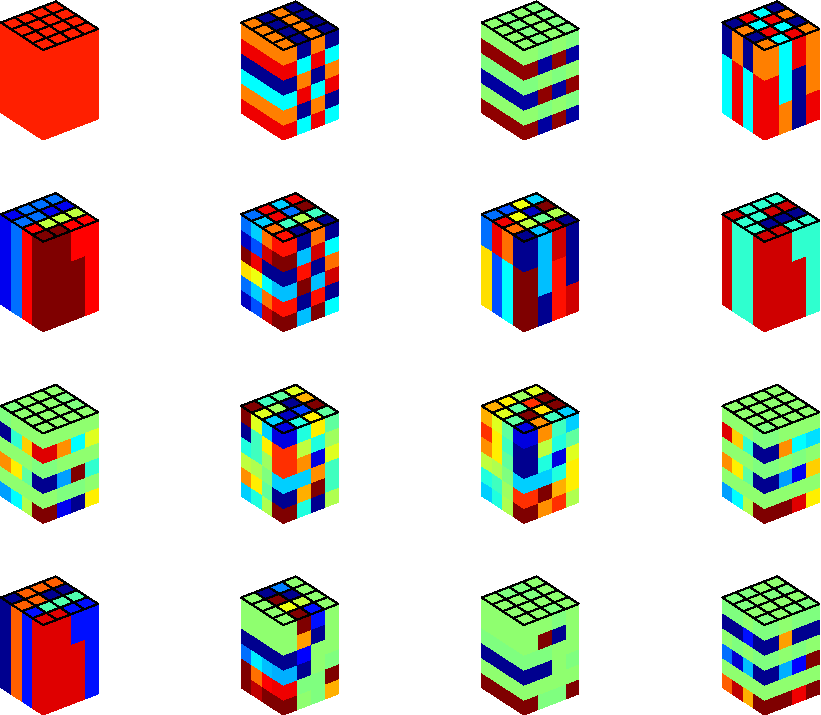
\includegraphics[width=0.45\columnwidth]{Fig/atom_dct}
\label{fig:atom_dct}}
   \subfigure[]{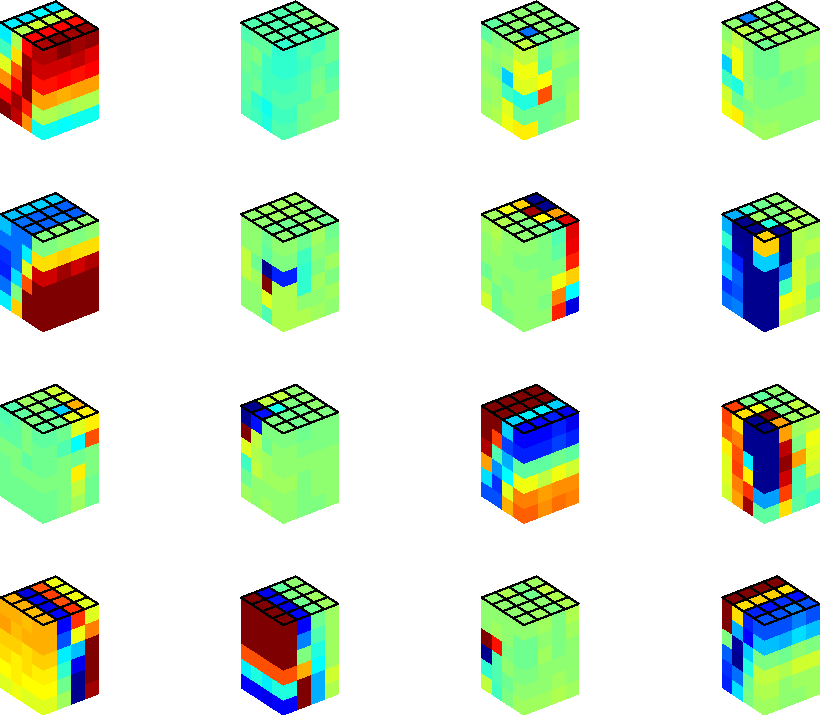
\includegraphics[width=0.45\columnwidth]{Fig/atom_ksvd}
   \label{fig:atom_ksvd}}\\
   \subfigure[]{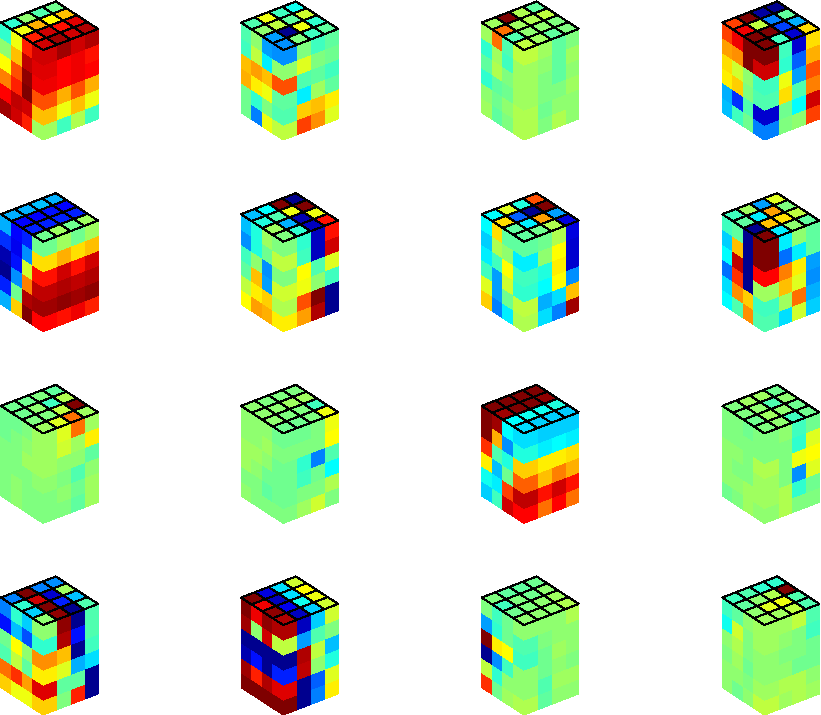
\includegraphics[width=0.45\columnwidth]{Fig/atom_ddtf}
   \label{fig:atom_ddtf}}
   \subfigure[]{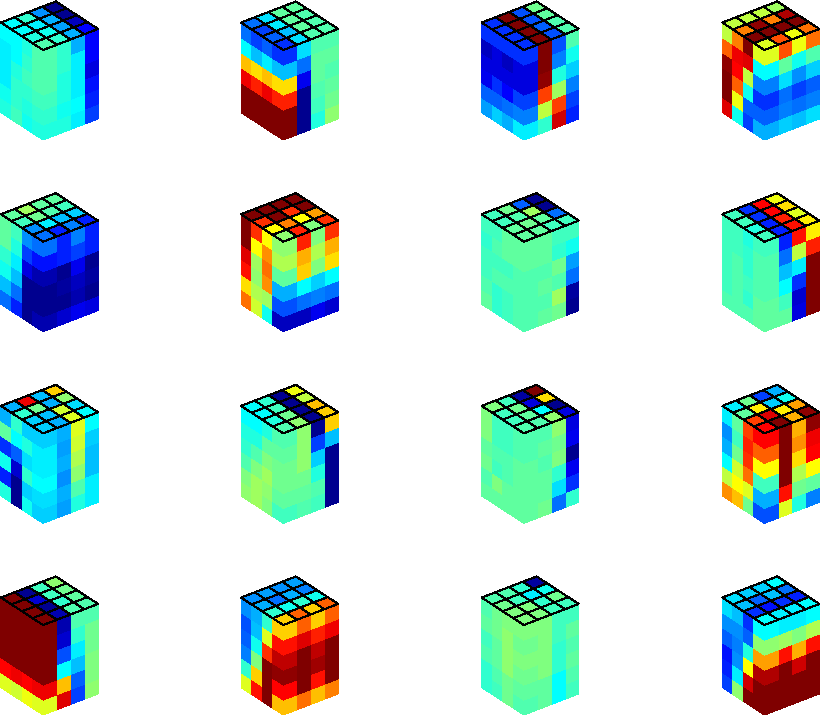
\includegraphics[width=0.45\columnwidth]{Fig/atom_sgk}
   \label{fig:atom_sgk}}
\caption{Comparison of different dictionary atoms. (a) Dictionary atoms of the discrete cosine transform. (b) Dictionary atoms of the KSVD method. (c) Dictionary atoms of the DDTF method.  (d) Dictionary atoms of the SGK method. }
\label{fig:atom_dct,atom_ksvd,atom_ddtf,atom_sgk}
\end{figure}

To date, the KSVD based method is one of the most widely used dictionary learning methods. However, the KSVD method requires computationally expensive dictionary update and sparse coding due to many singular value decomposition (SVD) and orthogonal matching pursuit (OMP) operations. The high computational cost of KSVD method limits its wide application in high-dimensional problems, e.g., 3D/5D seismic reconstruction. In this paper, we develop an efficient dictionary learning method based on a different learning model, which is referred to as the sequential generalized K-means (SGK) model \cite{sgk2013,yangkang2020sgk}. The SGK model is inspired from the work in \cite{sgk2013}, and is an extension of the previous work in \cite{yangkang2020sgk} for high-dimensional seismic reconstruction. The SGK model is applied to the patches created from the high-dimensional seismic data by the patching method \cite{wanghang2020}. Then, the computed denoised/reconstructed patches are concatenated to output the high-dimensional seismic data by the unpatching method \cite{wanghang2020}. We introduce in detail the accelerating principles in both dictionary update and sparse coding processes of the SGK method, and introduce the detailed algorithms. The computational speedup of the proposed SGK method is very appealing, i.e., at least 6 times speedup for small problems and more than 10 (or higher) times for larger problems. We use exclusive seismic data examples for both 3D and 5D reconstructions to demonstrate the comparable performance of the proposed method with the state-of-the-art KSVD method and the much accelerated computational performance. 


\section{Theory}
The traditional DL is usually realized by the KSVD method which includes two parts. The first step is to represent the signal with sparse coefficients by a given dictionary. The later one updates the dictionary based on the fixed sparse coefficients. These two steps are alternately carried out until the best representation of signals is obtained.

\subsection{Sparse coding}
We use $\mathbf{x}$ to represent the observed field data. After dividing it into different sample patches $\mathbf{x}_j$, the data used to train the dictionary can be expressed as $\mathbf{X}$ ($M\times N$) whose $j$th column is $\mathbf{x}_j$ ($M\times 1$). Assuming that the rearranged data can be sparsely represented by the matrix multiplication of the dictionary $\mathbf{D}^{n}$ ($M\times L$) and sparse coefficients $\mathbf{S}$ ($L\times N$). The superscript $n$ means that it is the generated dictionary after $n$th iteration. Each column of $\mathbf{D}^{n}$ stands for an atom that is variable in every iteration step. To make this representation relationship sensible, the three matrices should meet the following requirement:
\new{
\begin{equation}
\forall_{j}\mathbf{s}_j^{n}=\mathop{\text{argmin}}_{\mathbf{s}_j} \parallel \mathbf{X}-\mathbf{D}^{n}\mathbf{S} \parallel_{F}^{2},\,\,\text{s.t.}\,\, \forall_{j}\parallel \mathbf{s}_j \parallel_{0} \,\leq P.
\label{eq:eq1}
\end{equation}}
$\forall_{j}$ is a symbol meaning that it is suitable for all the $\mathbf{s}_j$. $\mathbf{s}_j$ ($L\times 1$) means the sparse coefficients of $j$th sample in $\mathbf{X}$, which also corresponds to the $j$th column of the sparse matrix $\mathbf{S}$. \new{Here, a sample in $\mathbf{X}$ means a column in $\mathbf{X}$. The matrix $\mathbf{X}$ is a collection of all available samples for learning.} $\parallel \cdot \parallel_{F}$ and $\parallel \cdot \parallel_{0}$ stand for the Frobenius norm and the $L_0$ norm, respectively. \old{$T$}\new{$P$} is a sparsity requirement that the number of non-zero elements in $\mathbf{s}_j$ should not exceed \old{$T$}\new{$P$}.

Solving above equation is a very difficult task because it is NP-hard. To directly find the precise solution is almost impossible without using tremendous computing resources. Therefore, OMP is proposed as an alternative approach to effectively find a suitable solution of sparse coefficients.

OMP algorithm can provide an optimal linear combination of the selected atoms to represent the signals. First, one can select an atom and find its corresponding sparse coefficient. Then, the residual signal is calculated and will be decomposed by the new atom and coefficient. This procedure keeps going until the requirement of \old{$T$}\new{$P$} non-zero coefficients is satisfied. 

\begin{figure}[htb!]
\centering
\subfigure[]{\includegraphics[width=0.30\columnwidth]{synth/Fig/synth-ksvd-simi}
\label{fig:synth-ksvd-simi}}
   \subfigure[]{\includegraphics[width=0.30\columnwidth]{synth/Fig/synth-ddtf-simi}
   \label{fig:synth-ddtf-simi}}
   \subfigure[]{\includegraphics[width=0.30\columnwidth]{synth/Fig/synth-sgk-simi}
   \label{fig:synth-sgk-simi}}
\caption{Similarity comparison of reconstructed data using (a) KSVD, (b) DDTF, and (c) SGK.}
\label{fig:synth-ksvd-simi,synth-ddtf-simi,synth-sgk-simi}
\end{figure}


\begin{figure}[htb!]
\centering
	\subfigure[]{\includegraphics[width=0.31\columnwidth]{synth/Fig/synth-s-clean}
	\label{fig:synth-s-clean}}
   \subfigure[]{\includegraphics[width=0.31\columnwidth]{synth/Fig/synth-s-noisy}
   \label{fig:synth-s-noisy}}
   \subfigure[]{\includegraphics[width=0.31\columnwidth]{synth/Fig/synth-s-obs}
   \label{fig:synth-s-obs}}\\
\subfigure[]{\includegraphics[width=0.31\columnwidth]{synth/Fig/synth-s-ksvd}
\label{fig:synth-s-ksvd}}
   \subfigure[]{\includegraphics[width=0.31\columnwidth]{synth/Fig/synth-s-ddtf}
   \label{fig:synth-s-ddtf}}
   \subfigure[]{\includegraphics[width=0.31\columnwidth]{synth/Fig/synth-s-sgk}
   \label{fig:synth-s-sgk}}
\caption{\new{2D slice comparison of the synthetic example. (a) Clean data. (b) Noisy data. (c) Observed data. (d) Reconstructed data using KSVD. (e) Reconstructed data using DDTF. (f) Reconstructed data using SGK.}}
\label{fig:synth-s-clean,synth-s-noisy,synth-s-obs,synth-s-ksvd,synth-s-ddtf,synth-s-sgk}
\end{figure}


\begin{figure}[htb!]
\centering
\subfigure[]{\includegraphics[width=\columnwidth]{synth/Fig/synth-ss}}
\caption{Single-trace comparison. The black line corresponds to the ground-truth solution. The green line corresponds to the noisy data. The pink line corresponds to the proposed method, which is closest to the black line. The red line corresponds to the KSVD method. The blue line corresponds to the DDTF method.}
\label{fig:synth-ss}
\end{figure}


\begin{figure}[htb!]
\centering
\subfigure[]{\includegraphics[width=0.30\columnwidth]{synth/Fig/synth-mssa}
\label{fig:synth-mssa}}
   \subfigure[]{\includegraphics[width=0.30\columnwidth]{synth/Fig/synth-mssasgk}
   \label{fig:synth-mssasgk}}
\caption{Reconstructed data using (a) MSSA (SNR=9.51 dB), and (b) SGK with (a) as the initialization model (SNR=12.22 dB).}
\label{fig:synth-mssa,synth-mssasgk}
\end{figure}


\subsection{Dictionary update via KSVD}

When one get the matrix of sparse coefficients after the sparse coding process, the dictionary should be updated to better approximate the data features. This new process can be expressed as:
\begin{equation}
\mathbf{D}^{n+1}=\mathop{\text{argmin}}_{\mathbf{D}} \parallel \mathbf{X}-\mathbf{D}\mathbf{S}^{n} \parallel_{F}^{2}.
\end{equation}
Note that the sparse coefficients are fixed in this step. This equation can be solved in the following form:
\begin{equation}
\begin{aligned}
\parallel \mathbf{X}-\mathbf{D}\mathbf{S} \parallel_{F}^{2}&=\parallel \mathbf{X}-\sum_{j=1}^{L} \mathbf{d}_{j}\mathbf{s}_{T}^{j} \parallel_{F}^{2}\\
&=\parallel \mathbf{X}-\sum_{j\neq k}^{L} \mathbf{d}_{j}\mathbf{s}_{T}^{j}-\mathbf{d}_{k}\mathbf{s}_{T}^{k} \parallel_{F}^{2}\\
&=\parallel \mathbf{Q}_{k}-\mathbf{d}_{k}\mathbf{s}_{T}^{k} \parallel_{F}^{2}
\end{aligned},
\label{eq:ksvd}
\end{equation}
where $\mathbf{d}_{j}$ is the $j$th column of dictionary $\mathbf{D}$. $\mathbf{s}_{T}^{k}$ is the $k$th row of sparse matrix $\mathbf{S}$. \new{Here, the subscript $T$ simply indicates a row vector.} $\mathbf{Q}_{k}$ is a $M\times N$ matrix representing the error between the real data and the sparse representation of atoms except the $k$th column.

By making the low-rank approximations of the two terms closer, the above equation can be solved and the atom $\mathbf{d}_{k}$ can be obtained. By repeating this procedure, all the atoms in $\mathbf{D}$ can be updated. It is worth mentioning that if $\mathbf{s}_{T}^{k}$ contains some zero elements, the equation needs to be changed into a more flexible form. That is to say, if the $m$th coefficient in $\mathbf{s}_{T}^{k}$ is 0, the $\mathbf{s}_{T}^{k}$ can be rewritten as $\mathbf{s}_{new}^{k}$ which discards the $m$th element and has the size of $1\times N_{new}$. The $\mathbf{Q}_{k}$ will also correspondingly delete the $m$th column and get the new size $M\times N_{new}$. \new{Deleting the $m$th column in $Q_k$ is required by the sparsity of the coefficient vector $s_T^k$. Suppose that the $m$th entry in $s_T^k$ is zero, if $m$th column in $Q_k$ is not deleted, then the $m$th entry of the updated $s_T^k$ after the rank-one decomposition ($\mathbf{Q}_k=\mathbf{d}_k\mathbf{s}_T^k$) will be filled with an non-zero value. It will damage the sparse structure of the coefficients vector $s_T^k$.} We use $\mathbf{Q}_{k}^{new}$ to stand for the new error term. The equation then can be formulated as:
\begin{equation}
\label{eq:err}
\parallel \mathbf{Q}_{k}-\mathbf{d}_{k}\mathbf{s}_{T}^{k} \parallel_{F}^{2}=\parallel \mathbf{Q}_{k}^{new}-\mathbf{d}_{k}\mathbf{s}_{new}^{k} \parallel_{F}^{2}.
\end{equation}
Solving this equation can save more calculation resources and generate the same satisfactory results as equation \ref{eq:ksvd}.

\subsection{Dictionary update via SGK}
Inspired from \cite{sgk2013}, here we introduce a different dictionary learning model:
\begin{equation}
\label{eq:modelsgk}
\forall_{j}\mathbf{s}_j^{n}=\mathop{\text{argmin}}_{\mathbf{s}_j} \parallel \mathbf{X}-\mathbf{D}^{n}\mathbf{S} \parallel_{F}^{2},\,\,\text{s.t.}\,\, \forall_{j} \mathbf{s}_j = \mathbf{e}_p,
\end{equation}
where $\mathbf{e}_p$ denotes a unit vector with $t$th element being 1 and other elements being 0. The constraint on $\mathbf{s}_j$, i.e., $\mathbf{s}_j = \mathbf{e}_p$, can be taken into consideration during the sparse coding process, which will be introduced in detail later. During the dictionary update processing, $\mathbf{D}$ needs to be updated like the way in KSVD method. It is natural to use the KSVD method here to solve the same dictionary update problem, but we turn to use a more efficient way, which is enabled due to the constraint of the unit vector applied onto the sparse coefficients.  Following equation \ref{eq:err}, we define the following objective function as:
\begin{equation}
\label{eq:obj}
J=\parallel \mathbf{Q}_{k}^{new}-\mathbf{d}_{k}\mathbf{s}_{new}^{k} \parallel_{F}^{2}.
\end{equation}
Taking the derivative of $J$ with respect to the coefficient vector $\mathbf{d}_k$ and setting it to zero, we obtain
\begin{equation}
\label{eq:err2}
\frac{\partial J}{\partial  \mathbf{d}_k}=-2( \mathbf{Q}_{k}^{new}-\mathbf{d}_{k}\mathbf{s}_{new}^{k} )(\mathbf{s}_{new}^{k})^T=0.
\end{equation}
The solution to equation \ref{eq:err2} can be given as:
\begin{equation}
\label{eq:err3}
\mathbf{d}_{k}=\mathbf{Q}_{k}^{new}(\mathbf{s}_{new}^{k})^T(\mathbf{s}_{new}^{k}(\mathbf{s}_{new}^{k})^T)^{-1}.
\end{equation}

Supposing there are $N^k$ non-zero elements in the row vector $\mathbf{s}_{new}^{k}$, then 
\begin{equation}
\label{eq:N}
\mathbf{s}_{new}^{k}(\mathbf{s}_{new}^{k})^T =N^k,
\end{equation}
then
\begin{equation}
\label{eq:err3}
\mathbf{d}_{k}=\frac{1}{N^k}\mathbf{Q}_{k}^{new}(\mathbf{s}_{new}^{k})^T.
\end{equation}
$\mathbf{Q}_{k}^{new}(\mathbf{s}_{new}^{k})^T$ can be expressed as:
\begin{equation}
\label{eq:Qk}
\begin{split}
\mathbf{Q}_{k}^{new}(\mathbf{s}_{new}^{k})^T & = \left( \mathbf{X}^{new}-\sum_{j\ne k}^{L} \mathbf{d}_{j}\mathbf{s}_{new}^{j} \right)(\mathbf{s}_{new}^{k})^T \\
&= \mathbf{X}^{new}(\mathbf{s}_{new}^{k})^T - \sum_{j\ne k}^{L} \mathbf{d}_{j}\mathbf{s}_{new}^{j}(\mathbf{s}_{new}^{k})^T.
\end{split}
\end{equation}
$\mathbf{X}^{new}$ has the same meaning as $\mathbf{Q}^{new}$, i.e., selecting only the columns in  $\mathbf{X}$ according to the non-zero element indices in $\mathbf{s}_{new}^k$. Since $\mathbf{s}_{new}^{k}$ is a row vector containing ones for all its entries, then $\mathbf{X}^{new}(\mathbf{s}_{new}^{k})^T$ denotes a summation across all the columns of $\mathbf{X}^{new}$:
\begin{equation}
\label{eq:sum}
 \mathbf{X}^{new}(\mathbf{s}_{new}^{k})^T = \sum_{i=1}^{N^k}\mathbf{x}_i.
\end{equation}
Since $\forall_{j} \mathbf{s}_j = \mathbf{e}_p$ (with $\mathbf{s}_j$ being a column vector), 
\begin{equation}
\label{eq:jk}
\forall_{j\ne k} \mathbf{s}_{new}^{j}(\mathbf{s}_{new}^{k})^T =0.
\end{equation}
Inserting equations \ref{eq:sum} and \ref{eq:jk} into equation \ref{eq:Qk}, and then into equation \ref{eq:err3}, we obtain
\begin{equation}
\label{eq:dk}
\mathbf{d}_{k}=\frac{1}{N^k}\sum_{i=1}^{N^k}\mathbf{x}_i.
\end{equation}
Equation \ref{eq:dk} corresponds to the whole process of dictionary update in the SGK method. It is intuitive that in SGK, the low-rank approximation of $k$th dictionary atom via singular value decomposition (SVD) operation has been replaced by a simple summation across the training samples.
\subsection{Sparse coding in SGK}
In the SGK method, sparse coding can also be efficiently accelerated  due to the special structure of the coefficient vectors, i.e., the unit vector. The traditional OMP algorithm solves the sparse coding problem recursively. Assuming that there are \old{$T$}\new{$P$} non-zero elements in each coefficient vector, the OMP algorithm iterates \old{$T$}\new{$P$} times to get the optimal representation of the target data sample by a linear combination of the dictionary atoms. Thus, the higher \old{$T$}\new{$P$} is, the larger speedup is due to the efficient sparse coding in SGK. Besides, calculation of the pseudo-inverse of the selected representative dictionary matrix in each iteration becomes larger when a larger number of non-zero coefficients need to be computed.  In the SGK algorithm, however, we only need one-time sparse coding. It means that we require one iteration instead of \old{$T$}\new{$P$} to compute the optimal sparse coefficients. We only need to select one atom in the dictionary that best matches the target data sample $\mathbf{x}_i$.  Thus, the sparse coding in SGK is also much accelerated.

The traditional OMP algorithm can be detailed in Algorithm \ref{alg:alg1}, where $I$ denotes a set of indices that correspond to the non-zero sparse coefficients. $\mathbf{D}_I$ denotes the representative dictionary matrix composed of the selected atoms. $(\mathbf{D}_I)^{\dagger}=(\mathbf{D}_I^T\mathbf{D}_I)^{-1}\mathbf{D}_I^T$ denotes the pseudo-inverse of the representative dictionary matrix.


\begin{algorithm}
   \caption{OMP algorithm in KSVD method}
   \textbf{Input:} Dictionary $\mathbf{D}$, Training samples $\mathbf{X}$, Sparse coding parameter $T$. \\
   \textbf{Output:} Sparse coefficients $\mathbf{S}$. 
    \begin{algorithmic}[1]
 \For{$n$ = $1,\cdots,N$}
 \State $n$th column in $\mathbf{X}$ is set as $\mathbf{x}$
 \State  $\mathbf{r}=\mathbf{x}$
 \For{\new{$p$ = $1,\cdots,P$}}
     \State $\hat{k}  = \displaystyle\arg\max_{k} |\mathbf{d}_k^T\mathbf{r}|$ 
     \State $I=(I,\hat{k})$
     \State $\mathbf{s}_I=\left(\mathbf{D}_I\right)^{\dagger}\mathbf{x}$
     \State $\mathbf{r}=\mathbf{x} - \mathbf{D}_I \mathbf{s}_I$ 
 \EndFor
  \State  $n$th column of $\mathbf{S}$ is set by $\mathbf{s}_I$ with the indices defined by $I$ chosen as the non-zero coefficients.
 \EndFor       
        
\end{algorithmic}
\label{alg:alg1}
\end{algorithm}
\new{$I = (I , \hat{k})$ means that each time one finds a sparse coefficient, the index $k$ is inserted into the index vector that is a collection of the indices of non-zero elements in the sparse coefficient vector.} As a comparison, the accelerated sparse coding algorithm in the SGK method can be detailed in Algorithm \ref{alg:alg2}.

\begin{algorithm}
   \caption{Sparse coding algorithm in SGK method}
   \textbf{Input:} Dictionary $\mathbf{D}$, Training samples $\mathbf{X}$. \\
   \textbf{Output:} Sparse coefficients $\mathbf{S}$. 
    \begin{algorithmic}[1]
 \For{$n$ = $1,\cdots,N$}
 \State $n$th column in $\mathbf{X}$ is set as $\mathbf{x}$
     \State $\hat{k}  = \displaystyle\arg\max_{k} |\mathbf{d}_k^T\mathbf{x}|$ 
  \State  $\hat{k}$th entry in $n$th column of $\mathbf{S}$ is set by $\mathbf{d}_k^T\mathbf{x}/(\mathbf{d}_k^T\mathbf{d}_k)$.
 \EndFor       
\end{algorithmic}
\label{alg:alg2}
\end{algorithm}


%\subsection{Comparison between KSVD, DDTF and SGK}


\subsection{Reconstruction based on the POCS method}
The reconstruction of seismic data can be expressed as the following inverse problem:
\begin{equation}
\label{eq:inv}
\mathbf{d}_{obs}= \mathbf{M}\mathbf{d},
\end{equation}
where $\mathbf{d}_{obs}$ is the observed incomplete data, $\mathbf{d}$ denotes the complete data to be reconstructed. $\mathbf{M}$ is the sampling operator. The structure of $\mathbf{M}$ has been introduced in many published papers, e.g., in \cite{mostafa2011}. We use an iterative POCS method to solve the inverse problem:
\begin{equation}
\label{eq:iter}
\mathbf{d}_{m+1} = \mathbf{M}\mathbf{d}_{obs} + (\mathbf{I}-\mathbf{M})\mathcal{F}(\mathbf{d}_m),
\end{equation}
where $m$ denotes iteration number, $\mathcal{F}$ denotes a reconstruction operator. In this paper, we use the dictionary learning based reconstruction operator, which can be expressed as:
\begin{equation}
\label{eq:Fdm}
\mathbf{F}(\mathbf{d}_m) = \mathcal{P}^{-1}(\hat{\mathbf{D}}\hat{\mathbf{S}}),
\end{equation}
where $\hat{\mathbf{D}}$ and $\hat{\mathbf{S}}$ are solution to the following problem:
\begin{equation}
\label{eq:pro}
\{\hat{\mathbf{D}},\hat{\mathbf{S}}\}=\arg\min_{\mathbf{D},\mathbf{S}} \parallel \mathcal{P}(\mathbf{d}_m)-\mathbf{D}\mathbf{S} \parallel_{F}^{2},\,\,\text{s.t.}\,\, \mathcal{C}(\mathbf{S}).
\end{equation}
$\mathcal{C}(\mathbf{S})$ denotes the constraint on the coefficient matrix $\mathbf{S}$, according to the KSVD method ($\forall_{j} \mathbf{s}_j \le P$) or the SGK method ($\forall_{j} \mathbf{s}_j = \mathbf{e}_p$). $\mathcal{P}$ and $\mathcal{P}^{-1}$ denote the patching and unpatching operators \cite{wanghang2020}, i.e., creating patches from the high-dimensional seismic data and reconstructing the high-dimensional seismic data from the patches. 

Equation \ref{eq:iter} is effective only when the seismic data contains no/little random nosie \cite{shuwei2016cs}. When there is strong random noise, we propose to use the following weighted POCS\new{-like} iteration:\old{$\mathbf{d}_{m+1} =\alpha_m\mathbf{M}\mathbf{d}_{obs} +  (1-\alpha_m) \mathbf{M} \mathcal{F}(\mathbf{d}_m)+(\mathbf{I}-\mathbf{M})\mathcal{F}(\mathbf{d}_m)$}
\begin{equation}
\label{eq:iter2}
\mathbf{d}_{m+1} =\alpha_m\mathbf{M}\mathbf{d}_{obs} +  (\mathbf{I}-\alpha_m\mathbf{M})  \mathcal{F}(\mathbf{d}_m),
\end{equation}
where $\alpha_m$ is a relaxing parameter that linearly decreases from 1 to 0 through iterations.

\begin{figure}[htb!]
\centering
\subfigure[]{\includegraphics[width=0.30\columnwidth]{hyper/Fig/hyper-clean}
\label{fig:hyper-clean}}
  \subfigure[]{\includegraphics[width=0.30\columnwidth]{hyper/Fig/hyper-noisy}
  \label{fig:hyper-noisy}}
  \subfigure[]{\includegraphics[width=0.30\columnwidth]{hyper/Fig/hyper-obs}
  \label{fig:hyper-obs}}
\caption{Synthetic example with hyperboloid events. (a) Clean data. (b) Noisy data (SNR=6.93 dB). (c) Observed data with 50\% randomly missing traces (SNR=2.21 dB).}
\label{fig:hyper-clean,hyper-noisy,hyper-obs}
\end{figure}


\begin{figure}[htb!]
\centering
\subfigure[]{\includegraphics[width=0.30\columnwidth]{hyper/Fig/hyper-mssa}
\label{fig:hyper-mssa}}
\subfigure[]{\includegraphics[width=0.30\columnwidth]{hyper/Fig/hyper-ksvd}
\label{fig:hyper-ksvd}}\\
  \subfigure[]{\includegraphics[width=0.30\columnwidth]{hyper/Fig/hyper-ddtf}
  \label{fig:hyper-ddtf}}
  \subfigure[]{\includegraphics[width=0.30\columnwidth]{hyper/Fig/hyper-sgk}
  \label{fig:hyper-sgk}}
\caption{Reconstructed data using (a) Rank-reduction method (SNR=9.68 dB), (b) KSVD (SNR=10.84 dB), (c) DDTF (SNR=11.45 dB), and (d) SGK (SNR=11.00 dB). All DL based methods use the result from the rank-reduction method as the initial model.}
\label{fig:hyper-mssa,hyper-ksvd,hyper-ddtf,hyper-sgk}
\end{figure}


\begin{figure}[htb!]
\centering
\subfigure[]{\includegraphics[width=0.30\columnwidth]{hyper/Fig/hyper-ksvd-simi}
\label{fig:hyper-ksvd-simi}}
  \subfigure[]{\includegraphics[width=0.30\columnwidth]{hyper/Fig/hyper-ddtf-simi}
  \label{fig:hyper-ddtf-simi}}
  \subfigure[]{\includegraphics[width=0.30\columnwidth]{hyper/Fig/hyper-sgk-simi}
  \label{fig:hyper-sgk-simi}}
\caption{Similarity comparison of reconstructed data using (a) KSVD, (b) DDTF, and (c) SGK.}
\label{fig:hyper-ksvd-simi,hyper-ddtf-simi,hyper-sgk-simi}
\end{figure}


\begin{figure}[htb!]
\centering
\subfigure[]{\includegraphics[width=0.31\columnwidth]{hyper/Fig/hyper-s-clean}
\label{fig:hyper-s-clean}}
  \subfigure[]{\includegraphics[width=0.31\columnwidth]{hyper/Fig/hyper-s-noisy}
  \label{fig:hyper-s-noisy}}
  \subfigure[]{\includegraphics[width=0.31\columnwidth]{hyper/Fig/hyper-s-obs}
  \label{fig:hyper-s-obs}}\\
\subfigure[]{\includegraphics[width=0.31\columnwidth]{hyper/Fig/hyper-s-ksvd}
\label{fig:hyper-s-ksvd}}
  \subfigure[]{\includegraphics[width=0.31\columnwidth]{hyper/Fig/hyper-s-ddtf}
  \label{fig:hyper-s-ddtf}}
  \subfigure[]{\includegraphics[width=0.31\columnwidth]{hyper/Fig/hyper-s-sgk}
  \label{fig:hyper-s-sgk}}
\caption{\new{2D slice comparison of the synthetic example. (a) Clean data. (b) Noisy data. (c) Observed data. (d) Reconstructed data using KSVD. (e) Reconstructed data using DDTF. (f) Reconstructed data using SGK.}}
\label{fig:hyper-s-clean,hyper-s-noisy,hyper-s-obs,hyper-s-ksvd,hyper-s-ddtf,hyper-s-sgk}
\end{figure}

%\begin{figure}[htb!]
%\centering
%\subfigure[]{\includegraphics[width=0.45\columnwidth]{hyper_regu/Fig/hyper2-obs}
%\label{fig:hyper2-obs}}
%  \subfigure[]{\includegraphics[width=0.45\columnwidth]{hyper_regu/Fig/hyper2-sgk}
%  \label{fig:hyper2-sgk}}
%\caption{\new{A reconstruction test for regularly missing traces. (a) Observed data. (b) Reconstructed data.}}
%\label{fig:hyper2-obs,hyper2-sgk}
%\end{figure}



\begin{figure}[htb!]
\centering
\subfigure[]{\includegraphics[width=0.31\columnwidth]{synth5d/Fig/syn5d-clean}
\label{fig:syn5d-clean}}
  \subfigure[]{\includegraphics[width=0.31\columnwidth]{synth5d/Fig/syn5d-noisy}
  \label{fig:syn5d-noisy}}
  \subfigure[]{\includegraphics[width=0.31\columnwidth]{synth5d/Fig/syn5d-obs}
  \label{fig:syn5d-obs}}\\
\subfigure[]{\includegraphics[width=0.31\columnwidth]{synth5d/Fig/syn5d-ksvd}
\label{fig:syn5d-ksvd}}
  \subfigure[]{\includegraphics[width=0.31\columnwidth]{synth5d/Fig/syn5d-ddtf}
  \label{fig:syn5d-ddtf}}
  \subfigure[]{\includegraphics[width=0.31\columnwidth]{synth5d/Fig/syn5d-sgk}
  \label{fig:syn5d-sgk}}
\caption{\new{Comparison of 5D seismic reconstruction in a common midpoint gather. (a) Clean data. (b) Noisy data (SNR=-0.65 dB). (c) Decimated data with 70\% randomly removed traces  (SNR=-0.21 dB). (d) Reconstructed data using KSVD  (SNR=6.58 dB). (e) Reconstructed data using DDTF  (SNR=3.22 dB). (f) Reconstructed data using SGK (SNR=6.58 dB).}}
\label{fig:syn5d-clean,syn5d-noisy,syn5d-obs,syn5d-ksvd,syn5d-ddtf,syn5d-sgk}
\end{figure}


\begin{figure}[htb!]
\centering
\subfigure[]{\includegraphics[width=0.31\columnwidth]{synth5d/Fig/syn5d-clean2}
\label{fig:syn5d-clean2}}
  \subfigure[]{\includegraphics[width=0.31\columnwidth]{synth5d/Fig/syn5d-noisy2}
  \label{fig:syn5d-noisy2}}
  \subfigure[]{\includegraphics[width=0.31\columnwidth]{synth5d/Fig/syn5d-obs2}
  \label{fig:syn5d-obs2}}\\
\subfigure[]{\includegraphics[width=0.31\columnwidth]{synth5d/Fig/syn5d-ksvd2}
\label{fig:syn5d-ksvd2}}
  \subfigure[]{\includegraphics[width=0.31\columnwidth]{synth5d/Fig/syn5d-ddtf2}
  \label{fig:syn5d-ddtf2}}
  \subfigure[]{\includegraphics[width=0.31\columnwidth]{synth5d/Fig/syn5d-sgk2}
  \label{fig:syn5d-sgk2}}
\caption{\new{Comparison of 5D seismic reconstruction in a common offset gather. (a) Clean data. (b) Noisy data (SNR=-0.65 dB). (c) Decimated data with 70\% randomly removed traces  (SNR=-0.21 dB). (d) Reconstructed data using KSVD  (SNR=6.58 dB). (e) Reconstructed data using DDTF  (SNR=3.22 dB). (f) Reconstructed data using SGK (SNR=6.58 dB).}}
\label{fig:syn5d-clean2,syn5d-noisy2,syn5d-obs2,syn5d-ksvd2,syn5d-ddtf2,syn5d-sgk2}
\end{figure}

\new{Despite of the highly incomplete sampling of the raw dataset, it is not difficult to learn dictionaries.  In the proposed framework, one can use two options to learn dictionaries from observed data. First, one can directly learn the dictionaries from incomplete data with missing traces. Secondly, one can also learn the dictionaries for initially reconstructed data (e.g., using a rank-based method). Both strategies will be illustrated later. }

\new{An interesting note is that enforcing $\mathbf{s}_j =\mathbf{e}_p$ ($P=1$) helps deriving the SVD-free dictionary updating scheme, as an averaged form of the training samples (e.g., in equation \ref{eq:dk}). $P=1$ is only required in the dictionary learning process. When applied to denoising or reconstruction, the sparse coding process expressed in equation \ref{eq:eq1}, (given the learned dictionary $\mathbf{D}$ from the SGK method), can be taken for the denoising or reconstruction purpose.}

\section{Examples}
To evaluate the performance of different methods, we use two metrics. The first one is the commonly used signal-to-noise ratio (SNR) metric, which is defined as:
\begin{equation}
\label{eq:snr}
\text{SNR}=20\log_{10}\frac{\Arrowvert \mathbf{d}_{true} \Arrowvert_2}{\Arrowvert \mathbf{d}_{true} -\mathbf{d}_{esti}\Arrowvert_2},
\end{equation}
where $\mathbf{d}_{true}$ denotes the ground-truth solution, i.e., clean data, and $\mathbf{d}_{esti}$ denotes the reconstructed/noisy data to estimate the SNR. Another quantitive metric is the local similarity metric \cite{fomel2007localattr,yangkang2015ortho}. A higher local similarity value between the clean and reconstructed/incomplete data means a more accurate reconstruction or a higher quality. All comparisons of computational costs are based on a Mac Pro Laptop with a 2.5 Ghz Intel Core i7 processor, and 16 GB LPDDR3 memory. In addition to the KSVD method, we also compare the performance of the proposed SGK method with the data-driven tight frame (DDTF) method \cite{siwei2016}.

We first test the performance of different algorithms to a 3D synthetic data with plane waves. The clean data of this example is plotted in Fig. \ref{fig:synth-clean}. We add some band-limited noise to the clean data and obtain the noisy data, as plotted in Fig. \ref{fig:synth-noisy}. We randomly remove 50\% of the total traces from the noisy data to generate the noisy and incomplete data, as shown in Fig. \ref{fig:synth-obs}. The SNRs of the noisy and incomplete data are -0.05 dB and -0.03 dB, respectively. The three reconstructed data using KSVD, DDTF, and the proposed methods are plotted in Fig. \ref{fig:synth-ksvd,synth-ddtf,synth-sgk}. The SNRs of KSVD, DDTF, and the proposed methods are 8.89 dB, 5.42 dB, 9.74 dB, respectively. It is clear that the SGK method obtains an obviously better result than the other two methods. Both KSVD and DDTF methods seem to leave significant residual noise while the SGK method causes the smallest amount of residual noise. Note that for all three methods, we use 10 iterations for dictionary update, and 12 iterations for the POCS method. The KSVD and DDTF methods use \new{$P=3$} for the sparse coding. The size of this dataset is $175\times 20\times20$. During the patching and unpatching steps, the patch size is $6\times 4\times 4$, and the shift size is the same for all three dimensions, i.e., 2 points. The KSVD method takes 313.41 s, DDTF method takes 255.05 s, and the proposed method takes only 51.30s, which is more than 6 times faster than the traditional KSVD method. The learned atoms of different methods are plotted in Fig. \ref{fig:atom_dct,atom_ksvd,atom_ddtf,atom_sgk}. The atoms of the initial dictionary refer to the discrete cosine transform, as plotted in Fig. \ref{fig:atom_dct}. The atoms learned from the KSVD, DDTF, and SGK methods are plotted in Figs. \ref{fig:atom_ksvd}, \ref{fig:atom_ddtf}, and \ref{fig:atom_sgk}, respectively. We further use the local similarity to evaluate the reconstruction performance. The local similarity between the ground-truth solution and all these three reconstructed data are shown in Fig. \ref{fig:synth-ksvd-simi,synth-ddtf-simi,synth-sgk-simi}, where the local similarity corresponding to the proposed method is obviously higher than the other two methods, indicating a higher reconstruction accuracy. The local similarity corresponding to the DDTF method seems to have lower values. A 2D slice comparison of different data are plotted in Fig. \ref{fig:synth-s-clean,synth-s-noisy,synth-s-obs,synth-s-ksvd,synth-s-ddtf,synth-s-sgk}.  The top row of Fig. \ref{fig:synth-s-clean,synth-s-noisy,synth-s-obs,synth-s-ksvd,synth-s-ddtf,synth-s-sgk} shows the clean data (left), noisy data (middle), and decimated data (right). The bottom row of Fig. \ref{fig:synth-s-clean,synth-s-noisy,synth-s-obs,synth-s-ksvd,synth-s-ddtf,synth-s-sgk} shows the results from KSVD (left), DDTF (middle), and SGK (right) methods. It is clear that the KSVD and SGK methods obtain obviously better results than the DDTF method, e.g., better signal preservation. A single-trace comparison is plotted in Fig. \ref{fig:synth-ss}. In Fig. \ref{fig:synth-ss}, the ground-truth solution is plotted as the black line. The green line corresponds to the noisy data, which clearly shows that the noise level is very strong. The results from the KSVD, DDTF, and SGK methods are plotted as pink, red, and blue lines, respectively. The pink line seems to be closest to the black line, demonstrating that the proposed method is best in preserving the amplitude as well as removing the strong random noise. All three methods use the discrete cosine transform as the initial dictionary atoms. The incomplete data are used directly as the initial guess in the POCS iteration. A better initial guess of the ground truth can help obtain a better reconstructed result in the proposed iterative framework. For example, we also conduct a benchmark comparison with the state-of-the-art multi-channel singular spectrum analysis (MSSA) method and show the result in Fig. \ref{fig:synth-mssa}, where the rank is chosen as three, since three corresponds to the number of plane-wave components in this dataset. The SNR of the MSSA result is 9.51 dB. Then, we use the result from the MSSA method as the initial model of the proposed framework, and obtain an even better result with a SNR equal to 12.22 dB, as shown in Fig. \ref{fig:synth-mssasgk}. 



\begin{figure}[htb!]
\centering
\subfigure[]{\includegraphics[width=0.30\columnwidth]{field/Fig/f-obs}
\label{fig:f-obs}}
\subfigure[]{\includegraphics[width=0.30\columnwidth]{field/Fig/f-ksvd}
\label{fig:f-ksvd}}\\
  \subfigure[]{\includegraphics[width=0.30\columnwidth]{field/Fig/f-ddtf}
  \label{fig:f-ddtf}}
  \subfigure[]{\includegraphics[width=0.30\columnwidth]{field/Fig/f-sgk}
  \label{fig:f-sgk}}
\caption{\new{3D Field data example. (a) Observed data. Reconstructed data using (b) KSVD, (c) DDTF, and (d) SGK.} }
\label{fig:f-obs,f-ksvd,f-ddtf,f-sgk}
\end{figure}

\begin{figure}[htb!]
\centering
\subfigure[]{\includegraphics[width=0.30\columnwidth]{field/Fig/f-s-obs0}
\label{fig:f-s-obs0}}
\subfigure[]{\includegraphics[width=0.30\columnwidth]{field/Fig/f-s-ksvd0}
\label{fig:f-s-ksvd0}}\\
  \subfigure[]{\includegraphics[width=0.30\columnwidth]{field/Fig/f-s-ddtf0}
  \label{fig:f-s-ddtf0}}
  \subfigure[]{\includegraphics[width=0.30\columnwidth]{field/Fig/f-s-sgk0}
  \label{fig:f-s-sgk0}}
\caption{2D slice comparison of the field data example. (a) Observed data. (b) Reconstructed data using KSVD. (c) Reconstructed data using DDTF. (d) Reconstructed data using SGK. The frame boxes are zoomed and shown in Figure \ref{fig:fz-obs,fz-ksvd,fz-ddtf,fz-sgk}. }
\label{fig:f-s-obs0,f-s-ksvd0,f-s-ddtf0,f-s-sgk0}
\end{figure}


\begin{figure}[htb!]
\centering
\subfigure[]{\includegraphics[width=0.30\columnwidth]{field/Fig/fz-obs}
\label{fig:fz-obs}}
\subfigure[]{\includegraphics[width=0.30\columnwidth]{field/Fig/fz-ksvd}
\label{fig:fz-ksvd}}\\
  \subfigure[]{\includegraphics[width=0.30\columnwidth]{field/Fig/fz-ddtf}
  \label{fig:fz-ddtf}}
  \subfigure[]{\includegraphics[width=0.30\columnwidth]{field/Fig/fz-sgk}
  \label{fig:fz-sgk}}
\caption{Zoomed 2D slice comparison of the field data example. (a) Observed data. (b) Reconstructed data using KSVD. (c) Reconstructed data using DDTF. (d) Reconstructed data using SGK. }
\label{fig:fz-obs,fz-ksvd,fz-ddtf,fz-sgk}
\end{figure}

\begin{figure}[htb!]
\centering
\subfigure[]{\includegraphics[width=0.45\columnwidth]{Fig/f5d-obs}
\label{fig:f5d-obs}}
\subfigure[]{\includegraphics[width=0.45\columnwidth]{Fig/f5d-ksvd}
\label{fig:f5d-ksvd}}\\
  \subfigure[]{\includegraphics[width=0.45\columnwidth]{Fig/f5d-ddtf}
  \label{fig:f5d-ddtf}}
  \subfigure[]{\includegraphics[width=0.45\columnwidth]{Fig/f5d-sgk}
  \label{fig:f5d-sgk}}
\caption{5D seismic reconstruction example. A common offset gather is displayed for comparison. The 3D common offset gather has been reformulated as 2D matrix. (a) Observed data with approximately 70\% missing traces. (b) Reconstructed data using KSVD. (c) Reconstructed data using DDTF. (d) Reconstructed data using SGK. }
\label{fig:f5d-obs,f5d-ksvd,f5d-ddtf,f5d-sgk}
\end{figure}


\begin{figure}[ht!]
\centering
\subfigure[]{\includegraphics[width=0.45\columnwidth]{Fig/z-obs}
\label{fig:z-obs}}
\subfigure[]{\includegraphics[width=0.45\columnwidth]{Fig/z-ksvd}
\label{fig:z-ksvd}}\\
  \subfigure[]{\includegraphics[width=0.45\columnwidth]{Fig/z-ddtf}
  \label{fig:z-ddtf}}
  \subfigure[]{\includegraphics[width=0.45\columnwidth]{Fig/z-sgk}
  \label{fig:z-sgk}}
\caption{Zoomed comparison of the 5D seismic reconstruction example. The zooming area is stressed by the frame boxes in Figure \ref{fig:f5d-obs,f5d-ksvd,f5d-ddtf,f5d-sgk}. (a) Observed data with approximately 70\% missing traces. (b) Reconstructed data using KSVD. (c) Reconstructed data using DDTF. (d) Reconstructed data using SGK. The SGK result is obviously better than the other two methods.}
\label{fig:z-obs,z-ksvd,z-ddtf,z-sgk}
\end{figure}

The second example is a 3D synthetic data with a hyperboloid event. The clean data are plotted in Fig. \ref{fig:hyper-clean}. The noisy data by adding band-limited noise and the decimated data by randomly removing 50\% traces are plotted in Figs. \ref{fig:hyper-noisy} and \ref{fig:hyper-obs}. The SNRs of the noisy and decimated data are 6.93 dB and 2.21 dB, respectively. In this test, the reconstructed data using four different methods, i.e., MSSA (9.68 dB), KSVD (10.84 dB), DDTF (11.45 dB), SGK (11.00 dB) methods, are plotted in Fig. \ref{fig:hyper-mssa,hyper-ksvd,hyper-ddtf,hyper-sgk}. \new{In this example, the MSSA is not applied in small windows. We use a rank parameter of 20 for the MSSA method.} All dictionary learning based methods use the result from the MSSA method as the initial model in the POCS method. Although in this case, the DDTF method obtains a higher SNR than the SGK method, the SGK method takes much less computing time. The size of this synthetic dataset is $50\times 32\times 32$. The patch size is $4\times 4 \times 4$. The shift size is 2 points for all dimensions  In this test, the sparse coding parameter is larger, i.e., \old{$T=30$}\new{$P=30$}, because of the curving structure. We use 10 iterations to update the dictionary in each method and use 10 iterations for the POCS method. The KSVD and DDTF method take 4,132.23s and 3,801.04s, respectively. The SGK method, however, takes 353.03s. The speedup compared with the KSVD method is almost 12 times. The local similarity maps between clean and reconstructed data for each dictionary learning method are plotted in Fig. \ref{fig:hyper-ksvd-simi,hyper-ddtf-simi,hyper-sgk-simi}, which demonstrates that the performance of the three dictionary learning methods are comparable. A 2D slice is extracted from each dataset and plotted in Fig. \ref{fig:hyper-s-clean,hyper-s-noisy,hyper-s-obs,hyper-s-ksvd,hyper-s-ddtf,hyper-s-sgk}, where the top row shows the clean data (left), noisy data (middle), and decimated data (right), and the bottom row shows the reconstructed data using KSVD (left), DDTF (middle), and SGK (right). The 2D slices demonstrate that all three dictionary learning methods obtain successful recovery of the hyperboloid seismic event. The DDTF and SGK methods are slightly better than the KSVD method in terms of residual noise. 
%\new{Based on this dataset, we also conduct a test for reconstructing regularly missing traces. As shown in Fig. \ref{fig:hyper2-obs,hyper2-sgk}, the proposed method is also effective in reconstructing the regularly missing traces.}

%\section{Discussions}


The third example is a 5D synthetic dataset. Since it is not convenient to plot 5D dataset, we extract a 3D cube (e.g., a common midpoint gather or a common offset gather) from the 5D datasets for comparison. A comparison of different datasets in the common midpoint domain is shown in Fig. \ref{fig:syn5d-clean,syn5d-noisy,syn5d-obs,syn5d-ksvd,syn5d-ddtf,syn5d-sgk}. The top row in Fig. \ref{fig:syn5d-clean,syn5d-noisy,syn5d-obs,syn5d-ksvd,syn5d-ddtf,syn5d-sgk} plots the clean data (left), the noisy data with band-limited random noise (middle), and the decimated data by randomly removing 70\% traces (right). The bottom row plots the reconstructed data by the KSVD (left), DDTF (middle), and the SGK (right) methods. The SNRs of the noisy and decimated data are -0.65 dB and -0.21 dB, respectively. After reconstruction, the KSVD, DDTF, and SGK methods obtain SNRs of 6.58 dB, 3.22 dB, and 6.58 dB, respectively. For this dataset, the SNR of the DDTF is however much lower than the other two methods, which indicates a somewhat unstable performance of the DDTF method. Note that we have tuned the parameters by a try-and-error method but could not obtain a better result for the DDTF method. When observing the reconstructed data in Fig. \ref{fig:syn5d-clean,syn5d-noisy,syn5d-obs,syn5d-ksvd,syn5d-ddtf,syn5d-sgk}, it also shows that the DDTF method causes obvious amplitude damages since the energy of the reconstructed seismic events is much weaker compared with the ground-truth solution shown in Fig. \ref{fig:syn5d-clean}. Both KSVD and SGK methods, however, are comparable and perform successfully. The size of this dataset is $100\times10\times10\times10\times10$. We use a sparse coding parameter \old{$T=3$}\new{$P=3$} for all dictionary learning methods. The patch size of the first dimension is 6 points and the patch sizes for all the spatial dimensions are 4 points. The shift sizes for all dimensions are all 2 points. 
We use 10 iterations for dictionary update and 5 iterations for the POCS reconstruction. In this test, the SGK method takes only 1,232.21s, while the KSVD method takes 7,348.99s and the DDTF method takes 6,503.32s.  The speedup is almost 6 times. In a similar way, Fig. \ref{fig:syn5d-clean2,syn5d-noisy2,syn5d-obs2,syn5d-ksvd2,syn5d-ddtf2,syn5d-sgk2} plots a comparison of different datasets in the common offset domain, where we can observe a similar phenomenon as in the common midpoint domain. 

The fourth example is a 3D field dataset. \new{Fig. \ref{fig:f-obs} shows the observed data with 56\% traces missing. There is a large gap (about 10 continuous traces) in the front slice. It is a post-stack dataset. The two space dimensions mean midpoint number in X and midpoint number in Y, respectively.} Figs. \ref{fig:f-ksvd}-\ref{fig:f-sgk} plot the reconstructed data using KSVD, DDTF, and SGK methods respectively. It is clear that all three dictionary learning methods obtain satisfactory results. The size of this dataset is $300\times 100\times 10$. Because of the complexity of this field dataset, we use a relatively high sparse-coding parameter, i.e., \old{$T=20$}\new{$P=20$}. We use 10 iterations for dictionary update and 5 iterations for the POCS reconstruction. Due to a larger \old{$T$}\new{$P$}, the KSVD and DDTF methods take a very long time, i.e., 6800.67 s for KSVD and 6300.34 s for DDTF. The SGK method, however, takes only 645.31 s, which is more than 10 times faster than the KSVD method. We extract a 2D slice from each dataset in Fig. \ref{fig:f-obs,f-ksvd,f-ddtf,f-sgk} and show the corresponding results in Fig. \ref{fig:f-s-obs0,f-s-ksvd0,f-s-ddtf0,f-s-sgk0}. We further zoom in the sections for a better evaluation of the reconstruction and show the zoomed data in Fig. \ref{fig:fz-obs,fz-ksvd,fz-ddtf,fz-sgk}. It is clear from Fig. \ref{fig:fz-obs,fz-ksvd,fz-ddtf,fz-sgk} that the proposed SGK method seems to obtain the best recovery of the shallow weak signals. The DDTF method, however, shows weakest energy of the shallow seismic events. \new{From this example, we also conclude that a continuously missing 10\% of the whole traces can be reconstructed with good performance.}

The final example is a 5D field dataset. \new{The four spatial dimensions of this field dataset are midpoint X, midpoint Y, offset X, and offset Y. This dataset has not gone through any pre-processing steps, except for the binning from irregular spatial coordinates onto regular grids. } Here, we extract a common offset gather from the 5D dataset and plot the common offset gather as a 2D matrix, which clearly shows the reconstruction performance. Fig. \ref{fig:f5d-obs} plots the observed 5D dataset in a 2D matrix, with a significant portion (roughly 70\%) of the data not recorded. Figs. \ref{fig:f5d-ksvd}-\ref{fig:f5d-sgk} show the reconstructed data using KSVD, DDTF, and SGK methods.  It is obvious that all three methods reconstruct most of the missing data and make the seismic waveforms much more coherent in the spatial dimension. However, in this dataset, the KSVD method seems to cause the worst result since the energy is obviously weaker compared with the other two methods. Besides, it fails in reconstructing the big gap as highlighted by the pink frame boxes. The size of this dataset is $100\times 4\times 4\times 20\times 20$. The patch size is $6\times 2 \times 2\times 4\times 4$. The shift size is 1 point for the first dimension and 2 points for all other dimensions. In this dataset, the sparse coding parameter \old{$T=3$}\new{$P=3$}. We use 10 iterations for dictionary update and 5 iterations for POCS reconstruction. The SGK method takes 1,203.53s, while the KSVD and DDTF take 8,766.97s and 7,793.12s, respectively. The speedup is about 7 times.  A zoomed comparison of different data is plotted in Fig. \ref{fig:z-obs,z-ksvd,z-ddtf,z-sgk} for a better view, which further demonstrates that the proposed SGK method seems to obtain the best result, and the DDTF method still causes some discontinuous reconstructed traces. From this test and the aforementioned numerical tests, it becomes clear that the KSVD and DDTF methods are less stable than the SGK method. It is difficult to predict which of the two methods (KSVD or DDTF) is better for a specific dataset, but we can conclude that the SGK method normally gives a stable and acceptable result with a high efficiency. \new{All the computation time comparisons are listed in Table \ref{tbl:timecomp}.}
%\new{
%\tabl{timecomp}{\new{Comparison of computation time among different dictionary learning methods.}}
% {
%    \begin{center}
%     \begin{tabular}{|c|c|c|c|} 
%	  \hline Tests & KSVD (s) &DDTF (s) & Proposed (s)			       		 \\ 
%	  \hline First synthetic & 313.41 &255.05 & 51.30 \\
%	  \hline Second synthetic & 4132.23 &3801.04 & 353.03 \\
%	  \hline Third synthetic  & 7348.99 & 6503.32 & 1232.21  \\
%	  \hline First field  &  6800.67 & 6300.34 &  645.31\\
%	  \hline Second field  & 8766.97 & 7793.12& 1203.53 \\
%      \hline 
%    \end{tabular} 
%   \end{center}
%}}
\new{
\begin{table}[h]
\caption{\new{Comparison of computation time among different dictionary learning methods.}}
\begin{center}
    \begin{tabular}{|c|c|c|c|} 
	  \hline Tests & KSVD (s) &DDTF (s) & Proposed (s)			       		 \\ 
	  \hline First synthetic & 313.41 &255.05 & 51.30 \\
	  \hline Second synthetic & 4132.23 &3801.04 & 353.03 \\
	  \hline Third synthetic  & 7348.99 & 6503.32 & 1232.21  \\
	  \hline First field  &  6800.67 & 6300.34 &  645.31\\
	  \hline Second field  & 8766.97 & 7793.12& 1203.53 \\
      \hline 
   \end{tabular} 
\end{center}
\label{tbl:timecomp}
\end{table}}


\section{Conclusions}
Dictionary learning (DL) uses an iterative process to update the sparse dictionary and the sparse coefficients in a data-driven way, thus is an adaptive approach in sparsity-promoting applications in seismic processing. We have introduced an efficient DL algorithm to deal with the computational bottleneck in high-dimensional seismic reconstructions based on the DL framework. Compared with the classic KSVD method, the proposed SGK method reduces the computational cost in the dictionary update step by replacing the SVD calculation with the calculation of mean of several input samples, and thus is less expensive. Besides, the SGK method saves significant cost by a special sparse coding that is free of the OMP algorithm, which further improves the computational efficiency. The proposed DL framework can not only be used as a standalone processing method, but also be combined with a conventional method. For example, it is applicable to learn the initial dictionary from the result of a first-step reconstruction method, e.g., the rank-reduction method, to obtain an even better result. We test the effectiveness and efficiency by both 3D and 5D examples, which both demonstrate promising performance. \new{Future research will focus on reconstructing regularly missing data based on the proposed method.}

\bibliographystyle{IEEEtran}
\bibliography{dl}



















%\begin{figure}[htb!]
%	\centering
%	\subfigure[]{\includegraphics[width=0.8\textwidth]{Fig/fig}}
%	\caption{Caption.}
%	\label{fig:fig}
%\end{figure}


%\begin{figure}[htb!]
%	\centering
%	\subfigure[]{\includegraphics[width=0.45\textwidth]{Fig/fig1}}\\
%    \subfigure[]{\includegraphics[width=0.45\textwidth]{Fig/fig2}}
%	\caption{(a) Caption a. (b) Caption b.}
%	\label{fig:fig1,fig2}
%\end{figure}

%\begin{table}[h]
%\caption{Table caption}
%\begin{center}
%     \begin{tabular}{|c|c|c|c|c|c|} 
%	  \hline Column1 (unit)  & Column2 (unit) & Column3 (unit) \\ 
%	  \hline 1 & 2  & 3 \\
%       \hline
%    \end{tabular} 
%\end{center}
%\label{tbl:table1}
%\end{table}





